\chapter{Inserimento in OpenStreetMaps}
\label{cap:PCLeOSM}
In questo capitolo si descriverà come sono state inserite le point cloud all'interno delle mappe e di come queste sono state messe a disposizione per l'utilizzo.

\section{OpenStreetMap}
\label{sez:OSM}

\begin{wrapfigure}{r}{0.3\linewidth}
    \vspace{-20pt}
        \begin{center}
            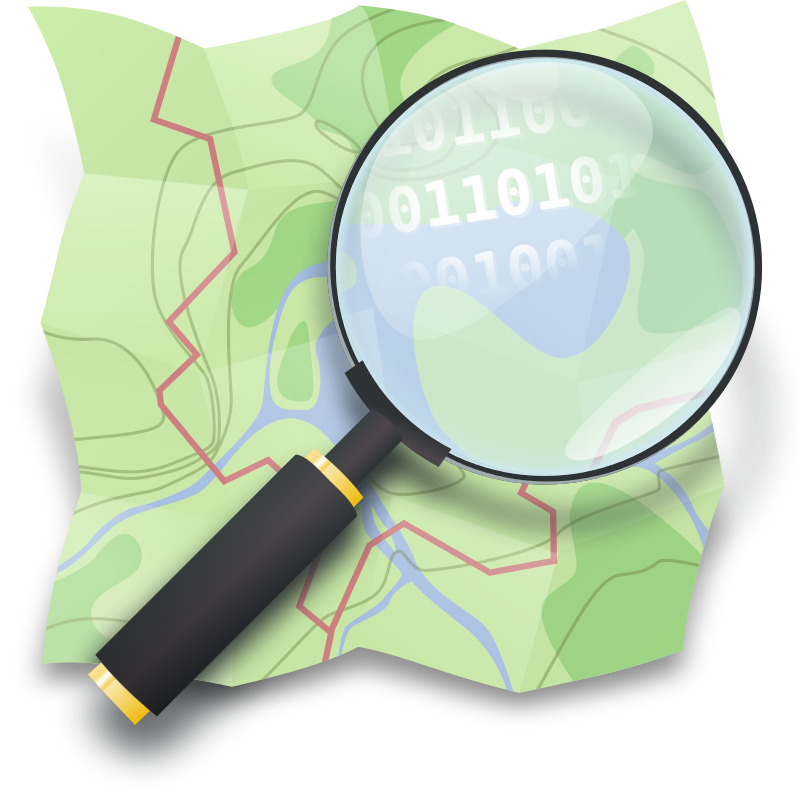
\includegraphics[width=0.2\textwidth]{Immagini/OSMLogo.png}
        \end{center}
    \vspace{-20pt}
    \caption{OSM Logo}
\label{fig:OSMLogo}
\end{wrapfigure}

OpenStreet Map\cite{OSM} è un'iniziativa per creare e fornire dati geografici a chiunque gestita dalla OpenStreetMap Foundation. Essa permette di contribuire, accedere ai dati e  ospitare una propria infrastruttura privata senza la necessità di appoggiarsi a infrastrutture chiuse e proprietarie.
OpenStreetMap è un database che utilizza un proprio formato di scambio dati basato su XML, tutti gli elementi che possono essere inseriti e che modellano la realtà sono di quattro tipologie: 
\begin{enumerate}
    \item punto (node): singolo punto. E' utilizzato per indicare oggetti puntuali.
    \begin{figure}[H]
    \centering
    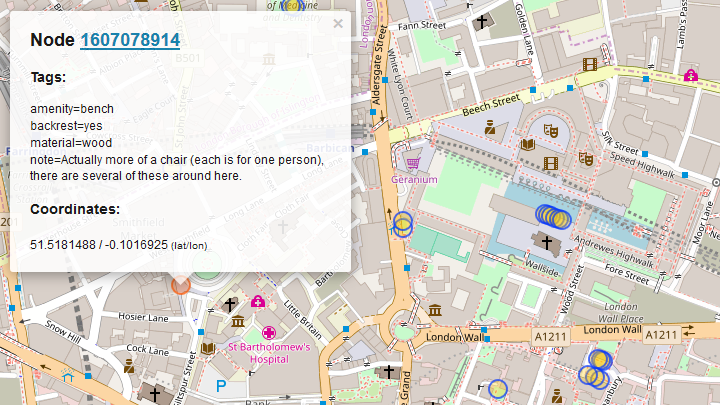
\includegraphics[width=0.5\textwidth]{Immagini/nodes.png}
    \caption{Node}
    \label{fig:OSMNode}
\end{figure}

    \item linea (way): un insieme di punti non chiuso, il percorso è un segmento tra punti che può descrivere oggetti che seguono una linea come vie, muri e simili.
    \begin{figure}[H]
    \centering
    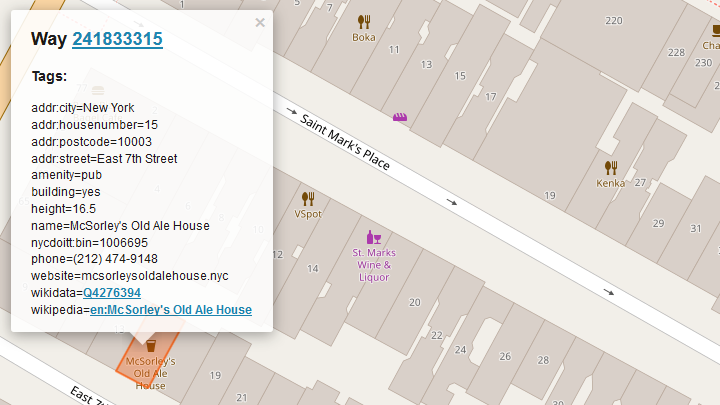
\includegraphics[width=0.5\textwidth]{Immagini/way.png}
    \caption{Way}
    \label{fig:OSMWay}
\end{figure}

    \item area (polygon): una linea chiusa ovvero un insieme di segmenti che si chiudono, è utilizzato per rappresentare oggetti che hanno un qualche tipo di area.
    \item relazione (relation): è un insieme degli elementi scritti sopra, esso consente di rappresentare oggetti complessi composti da un insieme di elementi.
    \begin{figure}[H]
    \centering
    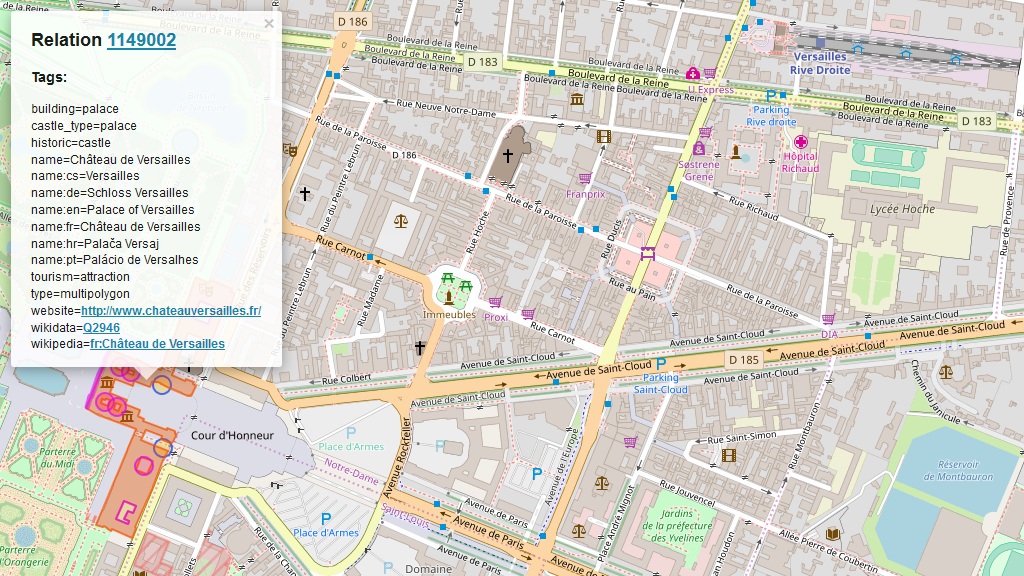
\includegraphics[width=0.5\textwidth]{Immagini/relation.png}
    \caption{Relation}
    \label{fig:OSMPolygon}
\end{figure}

\end{enumerate}{}
Nel progetto si sono manipolati elementi di tipo way e relation.
Per descrivere gli oggetti vengono utilizzate delle etichette (tag) che sono codificate secondo uno standard internazionale e sono composte da una tupla di elementi consistenti in una chiave (key) e un valore (value). Ogni oggetto dev'essere descritto da almeno un tag  principale per identificarlo ed è inoltre possibile aggiungerne di secondari che consentono di descrivere particolari proprietà. Il concetto di etichetta è stato utilizzato all'interno del progetto per consentire di aggiungere una chiave che possa descrivere la facciata di un edificio.

\section{JOSM}
\label{sez:JOSM}

\begin{wrapfigure}{r}{0.3\linewidth}
    \vspace{-20pt}
        \begin{center}
            
\includegraphics[width=0.2\textwidth]{Immagini/logoJOSM.png}
        \end{center}
    \vspace{-20pt}
    \caption{JOSM Logo}
\label{fig:JOSMLogo}
\end{wrapfigure}

JOSM\cite{josm} è un editor per OpenStreetMap(OSM) Open Source licenziato sotto GPL estensibile scritto in Java. Supporta l'editing avanzato delle mappe senza le limitazioni date dall'interfaccia web di OSM.
Consente inoltre il caricamento di tracciati GPX, l'utilizzo di immagini di backround, la modifica dei dati di OSM da sorgenti locali oltre che da sorgenti online. Consente inoltre di modificare tutte le tipologie di dato associate ad OSM e i loro tag.\newline
JOSM è stato scelto per la capacità di modificare in modo avanzato le mappe in particolare per poter modificare un'istanza locale di OSM e non dover modificare le mappe globali. 

\section{Docker}
\label{sez:Docker}

\begin{wrapfigure}{r}{0.3\linewidth}
    \vspace{-20pt}
        \begin{center}
            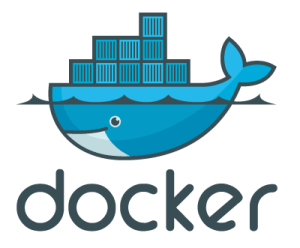
\includegraphics[width=0.2\textwidth]{Immagini/LogoDocker.png}
        \end{center}
    \vspace{-20pt}
    \caption{Docker Logo}
\label{fig:DockerLogo}
\end{wrapfigure}

Docker\cite{docker} è un progetto open-source nato per automatizzare il deployment di applicazioni all'interno di contenitore che in Docker si chiama Container, fornendo un livello ulteriore di astrazione grazie alla virtualizzazione a livello di sistema operativo concesso da Linux.\newline

Docker utilizza le funzionalità di isolamento delle risorse del kernel Linux, come cgroup e namespace per consentire a container indipendenti di coesistere sulla stessa istanza di Linux, evitando l'installazione e la manutenzione di una macchina virtuale (VM): i namespace del kernel Linux isolano ciò che l'applicazione può vedere dell'ambiente operativo, incluso l'albero dei processi, la rete, gli ID utente e i file system montati, mentre i cgroup forniscono l'isolamento delle risorse, inclusa la CPU, la memoria, i dispositivi di I/O a blocchi e la rete.\newline

Docker accede alle funzionalità di virtualizzazione del kernel Linux o direttamente utilizzando la libreria libcontainer, che è disponibile da Docker 0.9, o indirettamente attraverso libvirt, LXC o systemd-nspawn. I container condividono lo stesso kernel, ma ciascuno di essi può dover utilizzare una certa quantità di risorse, come la CPU, la memoria e l'I/O.\newline

\section{Inserimento nelle mappe}
\label{sez:insmap}
Per associare i singoli cluster agli edifici si è deciso di intervenire andando ad aggiungere una nuova etichetta agli edifici che presentavano il tag building.\\
Il tag aggiunto è denominato \textit{building:facade:pcl}, ad esso viene associato come valore l'url presso cui è salvato l'oggetto pcd che contiene la facciata dell'edificio.\\
L'aggiunta del tag è stata fatta manualmente attraverso l'utilizzo di \hyperref[sez:JOSM]{JOSM}, come si può vedere nella figura successiva.

\begin{figure}[H]
    \centering
    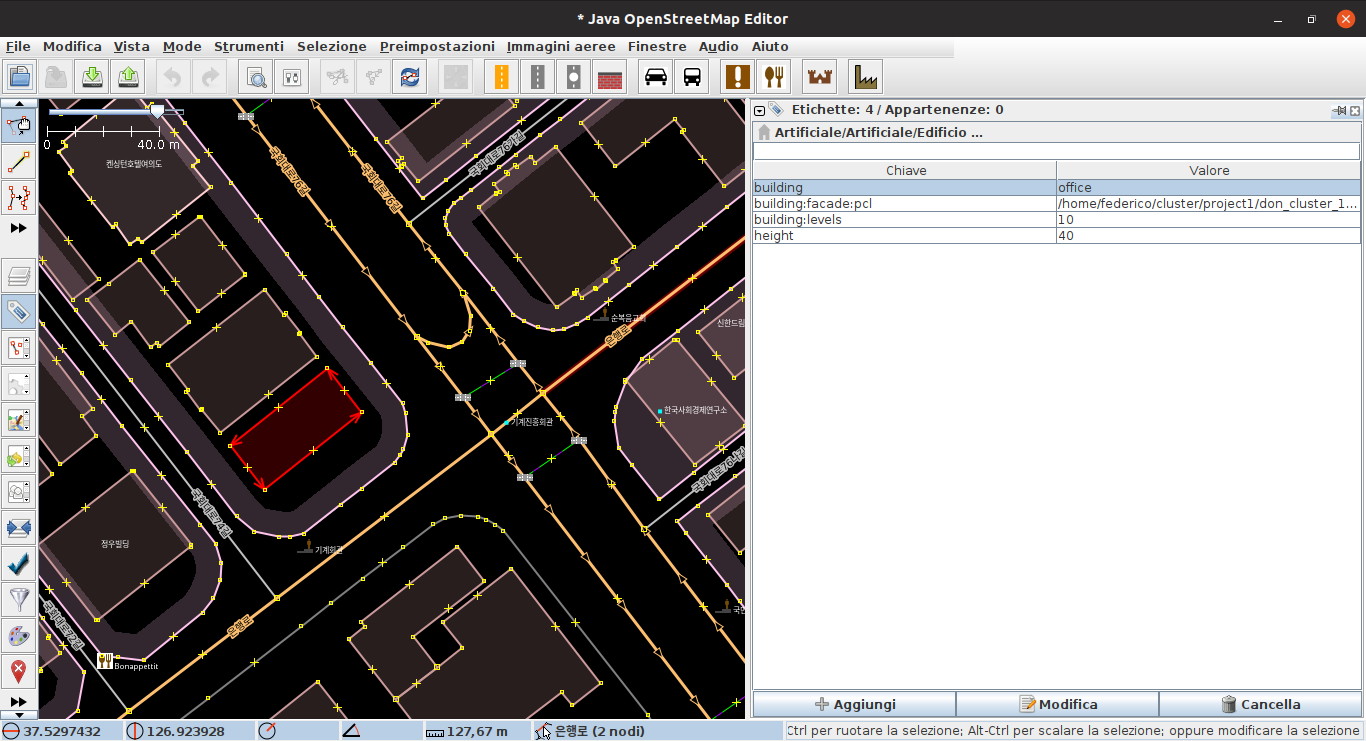
\includegraphics[width=0.9\textwidth]{Immagini/JOSMedit.png}
    \caption{Esempio di modifica di un edificio con JOSM}
    \label{fig:JOSMedit}
\end{figure}

Nel pannello di sinistra di può vedere il tracciato selezionato di tipo \textit{polygon} in quanto linea chiusa. 
Nel pannello di destra si possono invece evidenziare i tag associati allo specifico poligono, in particolare si può vedere che esso è un edificio e che vi è associato uno specifico cluster oltre che a dati di importanza secondaria come l'altezza dell'edifico o il numero di piani.
Il procedimento di associazione è stato ripetuto per ogni cluster precedentemente estratto, la mappa modificata è stata infine esportata per essere servita.

\subsection{Overpass API}
Per consentire l'estrazione delle informazioni si è deciso di utilizzare Overpass\cite{Overpass}.\\

Overpass API è un'API read-only che permette di servire i dati di regioni specifiche della mappa di OSM, funziona come un database, il client lancia una query all'API e riceve i dati che corrispondono alla query.\\

A differenza dell'API principale di OSM che è ottimizzata per l'editing, Overpass è ottimizzata per fornire pochi elementi in pochi secondi o fino a 10 milioni di elementi in pochi minuti entrambi filtrati da specifici criteri di ricerca. Funziona come backend per vari servizi.\\

Dal momento che non si voleva utilizzare la mappa globale ma una nostra versione modificata è stato necessario ospitare in locale un server Overpass, per poter far fronte alle difficoltà dovute all'utilizzo di versioni di librerie diverse e incompatibili tra loro si è deciso di utilizzare \hyperref[sez:Docker]{Docker} che permette di fare il deploy del server in un container portabile ed isolato.\\

Il container è stato costruito a partire da un container già esistente\cite{OverpassDocker} al quale sono state apportate modifiche per ottenere il seguente listato:
\begin{lstlisting}[caption={Dockerfile per OverpassAPI},captionpos=b,language=docker]

FROM ubuntu:16.04
RUN apt-get update 
RUN apt-get install -y apache2 vim
RUN apt-get install -y \
	autoconf \
	automake1.11 \
	expat \
	git \
	g++ \
	libtool \
	libexpat1-dev \
	make \
	zlib1g-dev \
	bzip2 \
	wget \
	liblz4-1 liblz4-dev
RUN apt-get clean && rm -rf /var/lib/apt/lists/*
RUN git clone https://github.com/drolbr/Overpass-API.git
WORKDIR /Overpass-API
#Checkout latest version
RUN git checkout $(git describe --abbrev=0 --tags)
#Configure
WORKDIR /Overpass-API/src
RUN \
	autoscan && \
	aclocal-1.11 && \
	autoheader && \
	libtoolize && \
	automake-1.11 --add-missing && \
	autoconf
#Compile
RUN \
	./configure --enable-lz4 CXXFLAGS="-O2" --prefix="`pwd`" && \
	make -j $(nproc --all)
COPY vhost_apache.conf /etc/apache2/sites-available
RUN a2enmod ext_filter cgi
RUN a2dissite 000-default.conf
RUN a2ensite vhost_apache.conf
WORKDIR /
COPY *.sh /
ADD www /www
RUN useradd overpass_api
CMD ["/run.sh"]
USER root
RUN chmod 777 /Overpass-API/src/bin/*
VOLUME "/overpass_DB"
EXPOSE 80
\end{lstlisting}
\vspace{5mm}
Il Dockerfile può essere diviso in 4 parti:
\begin{enumerate}
    \item Il pull dell'immagine dal dockerhub e l'installazione delle dipendenze necessarie.
    \item Il recupero del sorgente di Overpass API e la sua compilazione.
    \item La configurazione di apache per poter servire l'API.
    \item La definizione degli script da eseguire nel container e il binding con volumi che risiedono sul filesystem dell'ospite.
\end{enumerate}

Il binding è molto importante in quanto si è dovuto generare prima dell'esecuzione un database a cui l'API potesse accedere partendo dalla mappa personalizzata esportata in precedenza.\\
Dopo aver generato il DB di overpas attraverso degli strumenti dedicati messi a disposizione dal progetto OpenStreetMap, il container è stato lanciato nel seguente modo:

\begin{lstlisting}[language=bash]
docker run -d --restart=always -v ~/overpass_DB:/overpass_DB 
-p 5001:80 overpass_api 
\end{lstlisting}

\begin{figure}[H]
    \centering
    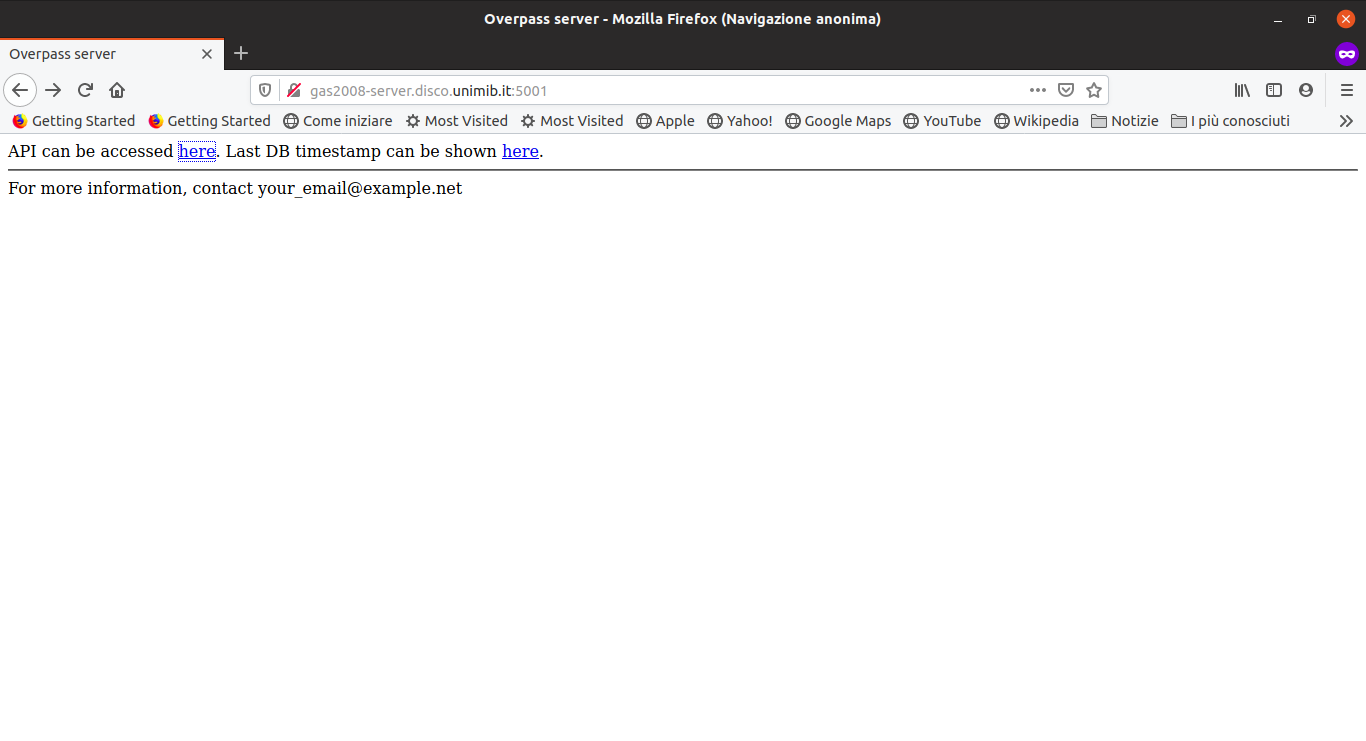
\includegraphics[width=0.7\textwidth]{Immagini/OverpassApiRunning.png}
    \caption{Overpass API in funzione}
    \label{fig:OverpassAPIRunning}
\end{figure}

E' ora possibile sottomettere query all'API utilizzando Overpass QL.
Grazie a Overpass QL possiamo andare ad effettuare query mirate, circoscritte all'interno di bounding box specifiche e andando a chiedere che il risultato contenga delle propietà specifiche
Una query può essere composta da:
\begin{itemize}
    \item Un'istruzione di query che inizia con \textit{"node", "way", "relation", "rel" , "nwr" (node+way+relation)}.
    \item Un' istruzione di output che inizia con \textit{"out"}. 
\end{itemize}

Le query consistono nel tipo di oggetto che dev'essere trovato:
\begin{lstlisting}
node
way
rel
\end{lstlisting}


seguito da almeno una condizione che deve descrivere l' oggetto da trovare ad esempio:\\
\begin{lstlisting}
["name"="Milano"]
\end{lstlisting}

In questo modo è possibile filtrare i singoli tag, cosa necessaria per il nostro progetto.
Infatti è stata costruita la seguente query:

\begin{lstlisting}[caption = {Query di Overpass QL}, captionpos=b,label={lst:OSMQuery}]
[out:json];
(way["building:facade:pcl"]
(37.52871919454917,
    126.91968441009521,
    37.531458875784935,
    126.9231390953064););
(._;>%;);
out meta;
\end{lstlisting}

Ciò consente di restituire tutti le way (e quindi anche i polygon) presenti all'interno del distretto di Yeongdeungpo a Seoul contenenti il tag "building:facade:pcl".

\begin{figure}[H]
    \centering
    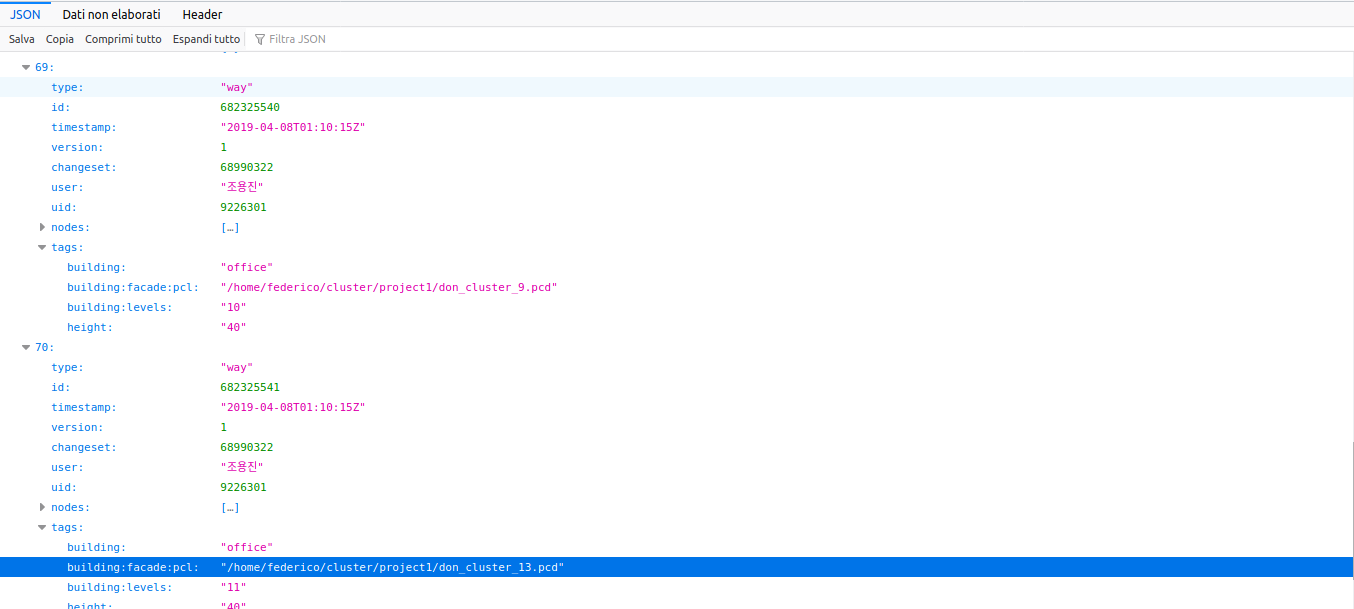
\includegraphics[width=0.7\textwidth]{Immagini/RisultatoQuery.png}
    \caption{Come si può vedere si trovano way con il tag building:facade:pcl presente}
    \label{fig:QueryResult}
\end{figure}

Il risultato della query verrà poi utilizzato per poter recuperare le point cloud quando sarà necessario il loro utilizzo durante il recupero da parte del componente di \hyperref[sez:RLE]{RLE} dedicato.  